%==============================================================================
% Additional files for: "NoiseInject: A Comprehensive Survey of Noise
% Robustness and Uncertainty Quantification in QSAR Models" —
% Journal of Cheminformatics submission.
%
% Compile this file separately from paper.tex.
% In Overleaf: Menu -> Settings -> Main document -> additional_files.tex,
% then Recompile, Download PDF, and use Preview / pdfseparate to split into
% Additional file 1.pdf, Additional file 2.pdf, ..., Additional file 11.pdf.
%
% ADDITIONAL FILE 1 IS GENERATED. Do not edit it here; edit
% models/model_defaults.py or the tuned-settings files and re-run
%   python scripts/generate_supp_table1.py --write
% Guard: python scripts/test_supp_table1.py
%
% Additional file 12, the representation-specific SVM kernel table, was removed
% on 2026-09-12: the support vector machine uses an RBF kernel on every
% representation (models/model_defaults.py, SKLEARN_DEFAULTS['svm']), so there
% are no representation-specific kernels to tabulate.
%==============================================================================

\documentclass[11pt]{article}

\usepackage[margin=1in]{geometry}
\usepackage{booktabs}
\usepackage{amsmath,amssymb,amsfonts}
\usepackage{graphicx}
\usepackage{enumitem}
\usepackage{caption}
\usepackage{float}% provides [H] to pin tables/figures exactly in place (no floating)
\usepackage{longtable}% multi-page tables that break across pages and stay under their title
\usepackage{microtype}

\graphicspath{{results/paper_figures/}}

\pagestyle{empty}
\setlength{\parindent}{0pt}
\setlength{\parskip}{0.5em}

\captionsetup{labelformat=empty,justification=raggedright,singlelinecheck=false}

\begin{document}

%==============================================================================
% Additional file 1 — Default hyperparameters (was Supp Table S1)
%==============================================================================

% BEGIN GENERATED Additional file 1 -- scripts/generate_supp_table1.py
% Do not edit between these two lines. Regenerate with
%   python scripts/generate_supp_table1.py --write

\begin{center}\Large\textbf{Additional file 1}\end{center}

{\small
\begin{longtable}{@{}p{5.0cm}p{5.0cm}p{4.6cm}@{}}
\caption{\textbf{Additional file 1, Table A: default hyperparameters for every model configuration in the study.}
Every value is read from \texttt{models/model\_defaults.py} at spec version 1.7.0, spec hash \texttt{9249926c38dc}, which is the file both the QM9 pipeline and the assay pipeline load their settings from. Every QM9 results row carries the spec version and the spec hash as two of its columns, so a QM9 table can be traced back to the settings that produced it; the three assay datasets are written by a second pipeline whose results files do not carry those two columns. The configuration list is the model roster the job generator submits. One setting is used for every representation and for every dataset, except where Table B gives a tuned replacement. The support vector machine uses an RBF kernel on every representation, so no result in this study carries a kernel that changes with the representation. Two values are not held in the shared spec and name their source file in the third column.}
\label{af1:hyperparameters}\\
\toprule
\textbf{Configuration} & \textbf{Hyperparameter} & \textbf{Default value} \\
\midrule
\endfirsthead
\toprule
\textbf{Configuration} & \textbf{Hyperparameter} & \textbf{Default value} \\
\midrule
\endhead
\multicolumn{3}{@{}l}{\textit{Shared by every neural network below}} \\
\midrule
Training, all networks & optimizer & adam \\
 & lr & 0.001 \\
 & weight\_decay & 0.0 \\
 & batch\_size & 32 \\
 & epochs & 100 \newline {\footnotesize\raggedright cap; early stopping usually reaches it first} \\
 & patience & 10 \newline {\footnotesize\raggedright epochs without a strictly better mean validation loss} \\
 & restore\_best\_weights & True \newline {\footnotesize\raggedright the reported fit is the best epoch, not the last} \\
 & val\_loss\_reduction & mean \\
 & improvement\_tolerance & 0.0 \\
 & mc\_passes & 100 \newline {\footnotesize\raggedright stochastic forward passes at inference} \\
 & standardise\_targets & True \newline {\footnotesize\raggedright fitted on training labels alone} \\
\midrule
\multicolumn{3}{@{}l}{\textit{Tree and boosting models}} \\
\midrule
RF \newline \footnotesize\texttt{rf} & n\_estimators & 100 \\
 & max\_depth & None \newline {\footnotesize\raggedright no limit} \\
 & min\_samples\_leaf & 5 \\
 & min\_samples\_split & 2 \\
 & max\_features & 0.3 \\
 & bootstrap & True \\
\addlinespace
RF300 \newline \footnotesize\texttt{rf300} & n\_estimators & 300 \\
 & max\_depth & None \newline {\footnotesize\raggedright no limit} \\
 & min\_samples\_leaf & 5 \\
 & min\_samples\_split & 2 \\
 & max\_features & 0.3 \\
 & bootstrap & True \\
\addlinespace
XGBoost \newline \footnotesize\texttt{xgboost} & n\_estimators & 100 \\
 & max\_depth & 6 \\
 & learning\_rate & 0.1 \\
 & subsample & 1.0 \\
 & colsample\_bytree & 1.0 \\
 & colsample\_bylevel & 1.0 \\
 & min\_child\_weight & 1 \\
 & gamma & 0.0 \\
 & reg\_alpha & 0.0 \\
 & reg\_lambda & 1.0 \\
\addlinespace
LightGBM \newline \footnotesize\texttt{lgb} & n\_estimators & 100 \\
 & learning\_rate & 0.1 \\
 & num\_leaves & 31 \\
 & max\_depth & $-1$ \newline {\footnotesize\raggedright no limit} \\
 & subsample & 1.0 \\
 & colsample\_bytree & 1.0 \\
 & min\_child\_samples & 20 \\
 & reg\_alpha & 0.0 \\
 & reg\_lambda & 0.0 \\
\addlinespace
NGBoost \newline \footnotesize\texttt{ngboost} & n\_estimators & 500 \\
 & learning\_rate & 0.01 \\
 & natural\_gradient & True \\
 & dist & Normal \newline {\footnotesize\raggedright ngboost.distns.Normal} \\
 & score & MLE \newline {\footnotesize\raggedright ngboost.scores.MLE, the log scoring rule} \\
 & minibatch\_frac & 1.0 \\
 & col\_sample & 1.0 \\
 & base\_max\_depth & 3 \newline {\footnotesize\raggedright depth of one boosting stage} \\
 & base\_criterion & friedman\_mse \\
 & early\_stopping\_rounds & 50 \newline {\footnotesize\raggedright stages without a better validation log likelihood} \\
 & use\_best\_iteration & True \newline {\footnotesize\raggedright predictions use the best stage, not every stage fitted} \\
 & ngboost\_ensemble\_seeds & 1 \newline {\footnotesize\raggedright 1 = one fit, no seed ensemble} \\
\addlinespace
QRF \newline \footnotesize\texttt{qrf} & n\_estimators & 300 \\
 & max\_depth & None \newline {\footnotesize\raggedright no limit} \\
 & min\_samples\_leaf & 5 \\
 & min\_samples\_split & 2 \\
 & max\_features & 0.3 \\
 & bootstrap & True \\
\midrule
\multicolumn{3}{@{}l}{\textit{Kernel models}} \\
\midrule
SVM \newline \footnotesize\texttt{svm} & C & 1.0 \\
 & gamma & scale \\
 & kernel & rbf \\
\addlinespace
GP \newline \footnotesize\texttt{gauche\_rbf} & kernel & rbf \newline {\footnotesize\raggedright set by this job, not by the shared spec} \\
 & likelihood\_noise & 0.001 \newline {\footnotesize\raggedright starting value; it is learned} \\
 & outputscale & 1.0 \\
 & apply\_outputscale & True \\
 & max\_train\_n & 5000 \newline {\footnotesize\raggedright molecules the process is fitted on; an exact Gaussian process is cubic in this. The test set is untouched and the number actually fitted is written into every results row} \\
 & fallback\_adam\_lr & 0.1 \newline {\footnotesize\raggedright used only when the standard fitter refuses the model} \\
 & fallback\_adam\_iters & 100 \newline {\footnotesize\raggedright used only when the standard fitter refuses the model} \\
 & single\_thread\_fit & False \newline {\footnotesize\raggedright a threading workaround, off since the environment check found one runtime} \\
 & init\_lengthscale\_from\_data & True \newline {\footnotesize\raggedright the RBF length scale starts at the median distance between training molecules, not at the library default} \\
 & lengthscale\_probe\_n & 500 \newline {\footnotesize\raggedright molecules sampled to estimate that median} \\
 & collapse\_fraction & 0.05 \newline {\footnotesize\raggedright a fit whose predictions vary by less than this fraction of the training label spread is recorded as collapsed rather than scored} \\
\addlinespace
GP-Tanimoto \newline \footnotesize\texttt{gauche} \newline \footnotesize run on ecfp4 only & kernel & tanimoto \newline {\footnotesize\raggedright set by this job, not by the shared spec} \\
 & likelihood\_noise & 0.001 \newline {\footnotesize\raggedright starting value; it is learned} \\
 & outputscale & 1.0 \\
 & apply\_outputscale & True \\
 & max\_train\_n & 5000 \newline {\footnotesize\raggedright molecules the process is fitted on; an exact Gaussian process is cubic in this. The test set is untouched and the number actually fitted is written into every results row} \\
 & fallback\_adam\_lr & 0.1 \newline {\footnotesize\raggedright used only when the standard fitter refuses the model} \\
 & fallback\_adam\_iters & 100 \newline {\footnotesize\raggedright used only when the standard fitter refuses the model} \\
 & single\_thread\_fit & False \newline {\footnotesize\raggedright a threading workaround, off since the environment check found one runtime} \\
 & init\_lengthscale\_from\_data & True \newline {\footnotesize\raggedright the RBF length scale starts at the median distance between training molecules, not at the library default} \\
 & lengthscale\_probe\_n & 500 \newline {\footnotesize\raggedright molecules sampled to estimate that median} \\
 & collapse\_fraction & 0.05 \newline {\footnotesize\raggedright a fit whose predictions vary by less than this fraction of the training label spread is recorded as collapsed rather than scored} \\
\addlinespace
GP-Hetero \newline \footnotesize\texttt{heteroscedastic\_gp} & kernel & rbf \newline {\footnotesize\raggedright set by this job, not by the shared spec} \\
 & likelihood\_noise & 0.001 \newline {\footnotesize\raggedright starting value; it is learned} \\
 & outputscale & 1.0 \\
 & apply\_outputscale & True \\
 & max\_train\_n & 5000 \newline {\footnotesize\raggedright molecules the process is fitted on; an exact Gaussian process is cubic in this. The test set is untouched and the number actually fitted is written into every results row} \\
 & fallback\_adam\_lr & 0.1 \newline {\footnotesize\raggedright used only when the standard fitter refuses the model} \\
 & fallback\_adam\_iters & 100 \newline {\footnotesize\raggedright used only when the standard fitter refuses the model} \\
 & single\_thread\_fit & False \newline {\footnotesize\raggedright a threading workaround, off since the environment check found one runtime} \\
 & init\_lengthscale\_from\_data & True \newline {\footnotesize\raggedright the RBF length scale starts at the median distance between training molecules, not at the library default} \\
 & lengthscale\_probe\_n & 500 \newline {\footnotesize\raggedright molecules sampled to estimate that median} \\
 & collapse\_fraction & 0.05 \newline {\footnotesize\raggedright a fit whose predictions vary by less than this fraction of the training label spread is recorded as collapsed rather than scored} \\
 & noise network hidden sizes & [64, 64] \newline {\footnotesize\raggedright models/models.py, not in the shared spec} \\
 & noise network output & Softplus, plus $10^{-4}$ \newline {\footnotesize\raggedright models/models.py, not in the shared spec} \\
 & Adam learning rate, process & 0.1 \newline {\footnotesize\raggedright models/models.py, not in the shared spec} \\
 & Adam learning rate, noise network & 0.001 \newline {\footnotesize\raggedright models/models.py, not in the shared spec} \\
 & noise network epochs & 100 \newline {\footnotesize\raggedright the shared epoch cap} \\
\midrule
\multicolumn{3}{@{}l}{\textit{Neural networks}} \\
\midrule
NN-$\alpha$ \newline \footnotesize\texttt{dnn} & hidden\_sizes & [128, 64] \\
 & dropout\_rate & 0.2 \\
 & activation & relu \\
\addlinespace
NN-$\beta$ \newline \footnotesize\texttt{mlp} & hidden\_size & 128 \\
 & num\_hidden\_layers & 2 \\
 & dropout\_rate & 0.2 \\
 & activation & relu \\
\addlinespace
BNN-$\alpha$ \newline \footnotesize\texttt{dnn\_bnn\_full} & hidden\_sizes & [128, 64] \\
 & dropout\_rate & 0.2 \\
 & activation & relu \\
 & bnn\_prior\_mu & 0.0 \\
 & bnn\_prior\_sigma & 0.1 \\
 & bnn\_kl\_weight & elbo \newline {\footnotesize\raggedright 1 / number of training molecules} \\
\addlinespace
BNN-$\beta$ \newline \footnotesize\texttt{mlp\_bnn\_full} & hidden\_size & 128 \\
 & num\_hidden\_layers & 2 \\
 & dropout\_rate & 0.2 \\
 & activation & relu \\
 & bnn\_prior\_mu & 0.0 \\
 & bnn\_prior\_sigma & 0.1 \\
 & bnn\_kl\_weight & elbo \newline {\footnotesize\raggedright 1 / number of training molecules} \\
\addlinespace
VBLL-$\alpha$ \newline \footnotesize\texttt{dnn\_bnn\_full\_variational} & hidden\_sizes & [128, 64] \\
 & dropout\_rate & 0.2 \\
 & activation & relu \\
 & vbll\_prior\_mu & 0.0 \\
 & vbll\_prior\_sigma & 1.0 \\
 & vbll\_init\_log\_sigma & $-3.0$ \\
 & vbll\_init\_log\_noise\_var & $-2.0$ \\
\addlinespace
VBLL-$\beta$ \newline \footnotesize\texttt{mlp\_bnn\_full\_variational} & hidden\_size & 128 \\
 & num\_hidden\_layers & 2 \\
 & dropout\_rate & 0.2 \\
 & activation & relu \\
 & vbll\_prior\_mu & 0.0 \\
 & vbll\_prior\_sigma & 1.0 \\
 & vbll\_init\_log\_sigma & $-3.0$ \\
 & vbll\_init\_log\_noise\_var & $-2.0$ \\
\addlinespace
VBLL-$\alpha$ (noise head) \newline \footnotesize\texttt{dnn\_bnn\_full\_variational\_hetero} & hidden\_sizes & [128, 64] \\
 & dropout\_rate & 0.2 \\
 & activation & relu \\
 & vbll\_prior\_mu & 0.0 \\
 & vbll\_prior\_sigma & 1.0 \\
 & vbll\_init\_log\_sigma & $-3.0$ \\
 & vbll\_init\_log\_noise\_var & $-2.0$ \\
 & observation noise & predicted per molecule \newline {\footnotesize\raggedright a variational noise head on the same features, started at the single-number value above} \\
\addlinespace
VBLL-$\beta$ (noise head) \newline \footnotesize\texttt{mlp\_bnn\_full\_variational\_hetero} & hidden\_size & 128 \\
 & num\_hidden\_layers & 2 \\
 & dropout\_rate & 0.2 \\
 & activation & relu \\
 & vbll\_prior\_mu & 0.0 \\
 & vbll\_prior\_sigma & 1.0 \\
 & vbll\_init\_log\_sigma & $-3.0$ \\
 & vbll\_init\_log\_noise\_var & $-2.0$ \\
 & observation noise & predicted per molecule \newline {\footnotesize\raggedright a variational noise head on the same features, started at the single-number value above} \\
\addlinespace
BNN-$\alpha$ (variance head) \newline \footnotesize\texttt{dnn\_bnn\_full\_mve} & hidden\_sizes & [128, 64] \\
 & dropout\_rate & 0.2 \\
 & activation & relu \\
 & bnn\_prior\_mu & 0.0 \\
 & bnn\_prior\_sigma & 0.1 \\
 & bnn\_kl\_weight & elbo \newline {\footnotesize\raggedright 1 / number of training molecules} \\
 & output head & value and log variance \newline {\footnotesize\raggedright two outputs} \\
 & loss & Gaussian negative log likelihood \\
 & log variance clamp & $[-10, 10]$ \newline {\footnotesize\raggedright scripts/loss\_functions.py, not in the shared spec} \\
\addlinespace
BNN-$\beta$ (variance head) \newline \footnotesize\texttt{mlp\_bnn\_full\_mve} & hidden\_size & 128 \\
 & num\_hidden\_layers & 2 \\
 & dropout\_rate & 0.2 \\
 & activation & relu \\
 & bnn\_prior\_mu & 0.0 \\
 & bnn\_prior\_sigma & 0.1 \\
 & bnn\_kl\_weight & elbo \newline {\footnotesize\raggedright 1 / number of training molecules} \\
 & output head & value and log variance \newline {\footnotesize\raggedright two outputs} \\
 & loss & Gaussian negative log likelihood \\
 & log variance clamp & $[-10, 10]$ \newline {\footnotesize\raggedright scripts/loss\_functions.py, not in the shared spec} \\
\bottomrule
\end{longtable}
}

\newpage

\begin{center}\Large\textbf{Additional file 1, continued}\end{center}

{\small
\begin{longtable}{@{}llll@{}}
\caption{\textbf{Additional file 1, Table B: the tuned settings that replace a default, and the four datasets they apply to.}
A setting is chosen once per model per dataset, not per representation, and is then used for all six representations: a two-way comparison across model and representation cannot be read if each cell carries its own hyperparameters. Only the Bayesian and variational networks are tuned; every other configuration in Table A trains at the default. A model with no row for a dataset kept the default on that dataset. Learning rates are printed to three significant figures; the source files hold the full value. Source files: \texttt{results/master\_tuned\_hyperparameters.json} for QM9 and \texttt{results/master\_tuned\_hyperparameters\_lab.json} for the three assay datasets.}
\label{af1:tuned}\\
\toprule
\textbf{Dataset} & \textbf{Configuration} & \textbf{Hyperparameter} & \textbf{Tuned value} \\
\midrule
\endfirsthead
\toprule
\textbf{Dataset} & \textbf{Configuration} & \textbf{Hyperparameter} & \textbf{Tuned value} \\
\midrule
\endhead
QM9 & NN-$\alpha$ & activation & tanh \\
 &  & hidden\_size1 & 64 \\
 &  & hidden\_size2 & 64 \\
\addlinespace
QM9 & BNN-$\alpha$ & activation & tanh \\
 &  & hidden\_size1 & 64 \\
 &  & hidden\_size2 & 64 \\
\addlinespace
QM9 & VBLL-$\alpha$ & activation & tanh \\
 &  & hidden\_size1 & 64 \\
 &  & hidden\_size2 & 64 \\
\addlinespace
QM9 & NN-$\beta$ & dropout\_rate & 0.401 \\
 &  & hidden\_size & 64 \\
 &  & lr & 0.00587 \\
 &  & num\_hidden\_layers & 3 \\
\addlinespace
QM9 & BNN-$\beta$ & dropout\_rate & 0.401 \\
 &  & hidden\_size & 64 \\
 &  & lr & 0.00587 \\
 &  & num\_hidden\_layers & 3 \\
\addlinespace
QM9 & VBLL-$\beta$ & dropout\_rate & 0.357 \\
 &  & hidden\_size & 64 \\
 &  & lr & 0.00119 \\
 &  & num\_hidden\_layers & 1 \\
\addlinespace
Caco-2 & NN-$\alpha$ & activation & tanh \\
 &  & hidden\_size1 & 64 \\
 &  & hidden\_size2 & 64 \\
\addlinespace
Caco-2 & BNN-$\alpha$ & activation & tanh \\
 &  & hidden\_size1 & 64 \\
 &  & hidden\_size2 & 64 \\
\addlinespace
Caco-2 & VBLL-$\alpha$ & activation & relu \\
 &  & hidden\_size1 & 64 \\
 &  & hidden\_size2 & 32 \\
\addlinespace
Caco-2 & NN-$\beta$ & dropout\_rate & 0.401 \\
 &  & hidden\_size & 64 \\
 &  & lr & 0.00587 \\
 &  & num\_hidden\_layers & 3 \\
\addlinespace
Caco-2 & BNN-$\beta$ & dropout\_rate & 0.401 \\
 &  & hidden\_size & 64 \\
 &  & lr & 0.00587 \\
 &  & num\_hidden\_layers & 3 \\
\addlinespace
hERG K$_i$ & NN-$\alpha$ & activation & tanh \\
 &  & hidden\_size1 & 64 \\
 &  & hidden\_size2 & 64 \\
\addlinespace
hERG K$_i$ & BNN-$\alpha$ & activation & tanh \\
 &  & hidden\_size1 & 64 \\
 &  & hidden\_size2 & 64 \\
\addlinespace
hERG K$_i$ & VBLL-$\alpha$ & activation & tanh \\
 &  & hidden\_size1 & 64 \\
 &  & hidden\_size2 & 64 \\
\addlinespace
hERG K$_i$ & NN-$\beta$ & dropout\_rate & 0.401 \\
 &  & hidden\_size & 64 \\
 &  & lr & 0.00587 \\
 &  & num\_hidden\_layers & 3 \\
\addlinespace
hERG K$_i$ & BNN-$\beta$ & dropout\_rate & 0.401 \\
 &  & hidden\_size & 64 \\
 &  & lr & 0.00587 \\
 &  & num\_hidden\_layers & 3 \\
\addlinespace
LogD & NN-$\alpha$ & activation & tanh \\
 &  & hidden\_size1 & 64 \\
 &  & hidden\_size2 & 64 \\
\addlinespace
LogD & BNN-$\alpha$ & activation & tanh \\
 &  & hidden\_size1 & 64 \\
 &  & hidden\_size2 & 64 \\
\addlinespace
LogD & VBLL-$\alpha$ & activation & tanh \\
 &  & hidden\_size1 & 256 \\
 &  & hidden\_size2 & 32 \\
\addlinespace
LogD & NN-$\beta$ & dropout\_rate & 0.401 \\
 &  & hidden\_size & 64 \\
 &  & lr & 0.00587 \\
 &  & num\_hidden\_layers & 3 \\
\addlinespace
LogD & BNN-$\beta$ & dropout\_rate & 0.401 \\
 &  & hidden\_size & 64 \\
 &  & lr & 0.00587 \\
 &  & num\_hidden\_layers & 3 \\
\addlinespace
LogD & VBLL-$\beta$ & dropout\_rate & 0.079 \\
 &  & hidden\_size & 128 \\
 &  & lr & 0.00011 \\
 &  & num\_hidden\_layers & 2 \\
\bottomrule
\end{longtable}
}

\newpage

\begin{center}\Large\textbf{Additional file 1, continued}\end{center}

{\small
\begin{longtable}{@{}llll@{}}
\caption{\textbf{Additional file 1, Table C: the 200 descriptors that make up the PDV representation.}
One entry is one feature of the vector, in the order the pipeline computes them. The list is fixed in the code rather than taken from RDKit's current default set, which grows between releases, so the same 200 features are built on every dataset and in every run. They were computed with RDKit 2022.09.5. Descriptors that return a non-finite value on a molecule have that value replaced by zero before the standardisation constants are computed. Source: \texttt{DEFAULT\_DESCRIPTOR\_LIST} in \texttt{scripts/process\_and\_train.py}.}
\label{af1:pdv}\\
\toprule
\endfirsthead
\toprule
\endhead
BalabanJ & NOCount & SlogP\_VSA7 & fr\_bicyclic \\
BertzCT & NumAliphaticCarbocycles & SlogP\_VSA8 & fr\_diazo \\
Chi0 & NumAliphaticHeterocycles & SlogP\_VSA9 & fr\_dihydropyridine \\
Chi0n & NumAliphaticRings & TPSA & fr\_epoxide \\
Chi0v & NumAromaticCarbocycles & VSA\_EState1 & fr\_ester \\
Chi1 & NumAromaticHeterocycles & VSA\_EState10 & fr\_ether \\
Chi1n & NumAromaticRings & VSA\_EState2 & fr\_furan \\
Chi1v & NumHAcceptors & VSA\_EState3 & fr\_guanido \\
Chi2n & NumHDonors & VSA\_EState4 & fr\_halogen \\
Chi2v & NumHeteroatoms & VSA\_EState5 & fr\_hdrzine \\
Chi3n & NumRadicalElectrons & VSA\_EState6 & fr\_hdrzone \\
Chi3v & NumRotatableBonds & VSA\_EState7 & fr\_imidazole \\
Chi4n & NumSaturatedCarbocycles & VSA\_EState8 & fr\_imide \\
Chi4v & NumSaturatedHeterocycles & VSA\_EState9 & fr\_isocyan \\
EState\_VSA1 & NumSaturatedRings & fr\_Al\_COO & fr\_isothiocyan \\
EState\_VSA10 & NumValenceElectrons & fr\_Al\_OH & fr\_ketone \\
EState\_VSA11 & PEOE\_VSA1 & fr\_Al\_OH\_noTert & fr\_ketone\_Topliss \\
EState\_VSA2 & PEOE\_VSA10 & fr\_ArN & fr\_lactam \\
EState\_VSA3 & PEOE\_VSA11 & fr\_Ar\_COO & fr\_lactone \\
EState\_VSA4 & PEOE\_VSA12 & fr\_Ar\_N & fr\_methoxy \\
EState\_VSA5 & PEOE\_VSA13 & fr\_Ar\_NH & fr\_morpholine \\
EState\_VSA6 & PEOE\_VSA14 & fr\_Ar\_OH & fr\_nitrile \\
EState\_VSA7 & PEOE\_VSA2 & fr\_COO & fr\_nitro \\
EState\_VSA8 & PEOE\_VSA3 & fr\_COO2 & fr\_nitro\_arom \\
EState\_VSA9 & PEOE\_VSA4 & fr\_C\_O & fr\_nitro\_arom\_nonortho \\
ExactMolWt & PEOE\_VSA5 & fr\_C\_O\_noCOO & fr\_nitroso \\
FpDensityMorgan1 & PEOE\_VSA6 & fr\_C\_S & fr\_oxazole \\
FpDensityMorgan2 & PEOE\_VSA7 & fr\_HOCCN & fr\_oxime \\
FpDensityMorgan3 & PEOE\_VSA8 & fr\_Imine & fr\_para\_hydroxylation \\
FractionCSP3 & PEOE\_VSA9 & fr\_NH0 & fr\_phenol \\
HallKierAlpha & RingCount & fr\_NH1 & fr\_phenol\_noOrthoHbond \\
HeavyAtomCount & SMR\_VSA1 & fr\_NH2 & fr\_phos\_acid \\
HeavyAtomMolWt & SMR\_VSA10 & fr\_N\_O & fr\_phos\_ester \\
Ipc & SMR\_VSA2 & fr\_Ndealkylation1 & fr\_piperdine \\
Kappa1 & SMR\_VSA3 & fr\_Ndealkylation2 & fr\_piperzine \\
Kappa2 & SMR\_VSA4 & fr\_Nhpyrrole & fr\_priamide \\
Kappa3 & SMR\_VSA5 & fr\_SH & fr\_prisulfonamd \\
LabuteASA & SMR\_VSA6 & fr\_aldehyde & fr\_pyridine \\
MaxAbsEStateIndex & SMR\_VSA7 & fr\_alkyl\_carbamate & fr\_quatN \\
MaxAbsPartialCharge & SMR\_VSA8 & fr\_alkyl\_halide & fr\_sulfide \\
MaxEStateIndex & SMR\_VSA9 & fr\_allylic\_oxid & fr\_sulfonamd \\
MaxPartialCharge & SlogP\_VSA1 & fr\_amide & fr\_sulfone \\
MinAbsEStateIndex & SlogP\_VSA10 & fr\_amidine & fr\_term\_acetylene \\
MinAbsPartialCharge & SlogP\_VSA11 & fr\_aniline & fr\_tetrazole \\
MinEStateIndex & SlogP\_VSA12 & fr\_aryl\_methyl & fr\_thiazole \\
MinPartialCharge & SlogP\_VSA2 & fr\_azide & fr\_thiocyan \\
MolLogP & SlogP\_VSA3 & fr\_azo & fr\_thiophene \\
MolMR & SlogP\_VSA4 & fr\_barbitur & fr\_unbrch\_alkane \\
MolWt & SlogP\_VSA5 & fr\_benzene & fr\_urea \\
NHOHCount & SlogP\_VSA6 & fr\_benzodiazepine & qed \\
\bottomrule
\end{longtable}
}

% END GENERATED Additional file 1

\newpage

%==============================================================================
% Additional file 2 — Pairwise model NDS correlations (was Supp Table S3)
%==============================================================================

\begin{center}\Large\textbf{Additional file 2}\end{center}

{\scriptsize
\begin{longtable}{llccc}
\caption{\textbf{Table S2: Pairwise Spearman rank correlations between model noise degradation slope (NDS) profiles on the QM9 HOMO--LUMO gap ($\rho \geq 0.95$).}
``Model A'' and ``Model B'' label each pair, both treated symmetrically. Checkmarks indicate pairs where one model was excluded from the ANOVA due to near-redundancy. Gauche (RBF) pairs omitted (all $\rho = 1.0$, $n = 6$, PDV-only artifact).}
\label{af2:model_redundancy}\\
\toprule
\textbf{Model A} & \textbf{Model B} & \textbf{$n$} & \textbf{$\rho$} & \textbf{Excluded} \\
\midrule
\endfirsthead
\toprule
\textbf{Model A} & \textbf{Model B} & \textbf{$n$} & \textbf{$\rho$} & \textbf{Excluded} \\
\midrule
\endhead
VBLL-$\beta$ & NGBoost & 18 & 0.998 &  \\
LightGBM & XGBoost & 46 & 0.998 &  \\
Gauche & VBLL-$\beta$ & 18 & 0.996 & \checkmark \\
QRF & RF & 40 & 0.995 & \checkmark \\
VBLL-$\alpha$ & LightGBM & 24 & 0.992 &  \\
RF & XGBoost & 46 & 0.989 &  \\
NGBoost & XGBoost & 40 & 0.988 &  \\
NGBoost & RF & 40 & 0.987 &  \\
LightGBM & RF & 46 & 0.986 &  \\
VBLL-$\beta$ & SVM & 24 & 0.986 &  \\
QRF & XGBoost & 40 & 0.986 & \checkmark \\
NGBoost & QRF & 34 & 0.986 & \checkmark \\
VBLL-$\alpha$ & NGBoost & 18 & 0.986 &  \\
VBLL-$\alpha$ & XGBoost & 24 & 0.984 &  \\
LightGBM & NGBoost & 40 & 0.984 &  \\
LightGBM & QRF & 40 & 0.984 & \checkmark \\
VBLL-$\alpha$ & VBLL-$\beta$ & 24 & 0.983 &  \\
NN-$\alpha$ & NN-$\beta$ & 52 & 0.983 &  \\
LightGBM & SVM & 46 & 0.982 &  \\
BNN-$\beta$ & SVM & 34 & 0.981 &  \\
VBLL-$\alpha$ & SVM & 24 & 0.979 &  \\
BNN-$\alpha$ & VBLL-$\beta$ & 24 & 0.979 &  \\
VBLL-$\alpha$ & QRF & 24 & 0.978 & \checkmark \\
SVM & XGBoost & 46 & 0.978 &  \\
BNN-$\alpha$ & BNN-$\beta$ & 36 & 0.977 &  \\
BNN-$\alpha$ & SVM & 34 & 0.976 &  \\
VBLL-$\alpha$ & Gauche & 18 & 0.975 & \checkmark \\
VBLL-$\alpha$ & RF & 24 & 0.975 &  \\
QRF & SVM & 40 & 0.974 & \checkmark \\
BNN-$\alpha$ & VBLL-$\alpha$ & 24 & 0.974 &  \\
LightGBM & VBLL-$\beta$ & 24 & 0.973 &  \\
VBLL-$\alpha$ & BNN-$\beta$ & 24 & 0.972 &  \\
Gauche & SVM & 40 & 0.972 & \checkmark \\
Gauche & XGBoost & 44 & 0.970 & \checkmark \\
NGBoost & SVM & 40 & 0.970 &  \\
NN-$\alpha$ & BNN-$\beta$ & 36 & 0.970 &  \\
Gauche & LightGBM & 42 & 0.969 & \checkmark \\
RF & SVM & 46 & 0.969 &  \\
BNN-$\beta$ & VBLL-$\beta$ & 24 & 0.968 &  \\
VBLL-$\beta$ & QRF & 24 & 0.966 & \checkmark \\
NN-$\alpha$ & BNN-$\alpha$ & 36 & 0.965 &  \\
VBLL-$\beta$ & XGBoost & 24 & 0.965 &  \\
NN-$\beta$ & SVM & 46 & 0.962 &  \\
NN-$\alpha$ & SVM & 46 & 0.960 &  \\
Gauche & NGBoost & 34 & 0.959 & \checkmark \\
LightGBM & BNN-$\beta$ & 36 & 0.959 &  \\
BNN-$\alpha$ & NN-$\beta$ & 36 & 0.958 &  \\
BNN-$\alpha$ & QRF & 28 & 0.956 & \checkmark \\
Gauche & QRF & 34 & 0.956 & \checkmark \\
VBLL-$\beta$ & RF & 24 & 0.955 &  \\
Gauche & RF & 40 & 0.954 & \checkmark \\
BNN-$\beta$ & XGBoost & 34 & 0.953 &  \\
BNN-$\beta$ & QRF & 28 & 0.952 & \checkmark \\
NN-$\alpha$ & VBLL-$\beta$ & 24 & 0.952 &  \\
NN-$\beta$ & BNN-$\beta$ & 36 & 0.952 &  \\
BNN-$\alpha$ & LightGBM & 36 & 0.951 &  \\
NN-$\beta$ & VBLL-$\beta$ & 24 & 0.950 &  \\
BNN-$\alpha$ & Gauche & 30 & 0.950 & \checkmark \\
\bottomrule
\end{longtable}}

\newpage

%==============================================================================
% Additional file 3 — Pairwise representation NDS correlations (was Supp Table S4)
%==============================================================================

\begin{center}\Large\textbf{Additional file 3}\end{center}

{\scriptsize
\begin{longtable}{llccc}
\caption{\textbf{Table S3: Pairwise Spearman rank correlations between representation noise degradation slope (NDS) profiles on the QM9 HOMO--LUMO gap.}
``Rep A'' and ``Rep B'' label each pair of molecular representations, both treated symmetrically. Checkmarks indicate pairs where one representation was excluded from the ANOVA.}
\label{af3:rep_redundancy}\\
\toprule
\textbf{Rep.\ A} & \textbf{Rep.\ B} & \textbf{$n$} & \textbf{$\rho$} & \textbf{Excluded} \\
\midrule
\endfirsthead
\toprule
\textbf{Rep.\ A} & \textbf{Rep.\ B} & \textbf{$n$} & \textbf{$\rho$} & \textbf{Excluded} \\
\midrule
\endhead
ECFP4 & Morgan & 60 & 0.995 & \checkmark \\
MHGGNN & Morgan & 48 & 0.994 & \checkmark \\
Rand.~SMILES & SMILES & 16 & 0.994 & \checkmark \\
Rand.~SMILES & SNS & 16 & 0.994 & \checkmark \\
ECFP4 & MHGGNN & 54 & 0.993 &  \\
ECFP4 & SNS & 56 & 0.992 & \checkmark \\
Morgan & SNS & 52 & 0.992 & \checkmark \\
MHGGNN & SNS & 44 & 0.991 & \checkmark \\
PDV & ECFP4 & 72 & 0.990 &  \\
PDV & MHGGNN & 48 & 0.989 &  \\
SMILES & SNS & 52 & 0.988 & \checkmark \\
Morgan & Rand.~SMILES & 16 & 0.988 & \checkmark \\
Morgan & SMILES & 54 & 0.988 & \checkmark \\
PDV & Morgan & 54 & 0.986 & \checkmark \\
PDV & Rand.~SMILES & 12 & 0.986 & \checkmark \\
PDV & SNS & 50 & 0.984 & \checkmark \\
ECFP4 & SMILES & 72 & 0.984 &  \\
Mol2Vec & Morgan & 48 & 0.982 & \checkmark \\
MHGGNN & Mol2Vec & 54 & 0.982 &  \\
ECFP4 & Mol2Vec & 54 & 0.982 &  \\
PDV & PDV (binary) & 72 & 0.980 & \checkmark \\
MHGGNN & SMILES & 48 & 0.980 &  \\
PDV & Mol2Vec & 48 & 0.979 &  \\
ECFP4 & Rand.~SMILES & 16 & 0.979 & \checkmark \\
PDV & SMILES & 66 & 0.978 &  \\
MHGGNN & PDV (binary) & 54 & 0.972 & \checkmark \\
Mol2Vec & SNS & 44 & 0.969 & \checkmark \\
Mol2Vec & SMILES & 48 & 0.966 &  \\
ECFP4 & PDV (binary) & 78 & 0.965 & \checkmark \\
Morgan & PDV (binary) & 60 & 0.962 & \checkmark \\
PDV (binary) & SNS & 56 & 0.961 & \checkmark \\
Mol2Vec & PDV (binary) & 54 & 0.956 & \checkmark \\
MHGGNN & Rand.~SMILES & 16 & 0.956 & \checkmark \\
PDV (binary) & SMILES & 72 & 0.941 & \checkmark \\
PDV (binary) & Rand.~SMILES & 16 & 0.929 & \checkmark \\
Mol2Vec & Rand.~SMILES & 16 & 0.891 & \checkmark \\
\bottomrule
\end{longtable}}

\newpage

%==============================================================================
% Additional file 4 — ICC(1,1) (was Supp Table S5)
%==============================================================================

\begin{center}\Large\textbf{Additional file 4}\end{center}

\begin{table}[H]
\centering
\caption{\textbf{Table S4: Intraclass correlation coefficients (ICC(1,1)) for model pairs with ICC $\geq 0.5$, assessing within-family consistency of noise degradation slope (NDS) profiles on the QM9 HOMO--LUMO gap.}
ICC(1,1) measures the proportion of total variance attributable to between-configuration differences; values near 1.0 indicate that two models rank configurations almost identically. Lower (more negative) NDS indicates faster degradation under noise. The Family column groups each pair: ``Tree'' (both tree-based), ``$\alpha$/$\beta$'' (architecture-pair partners such as BNN-$\alpha$/BNN-$\beta$), ``$\alpha$'' (both share the $\alpha$ neural-network backbone), or ``Cross'' (cross-family pair).}
\label{af4:icc}
\small
\begin{tabular}{llcccc}
\toprule
\textbf{Model A} & \textbf{Model B} & \textbf{$n$} & \textbf{ICC(1,1)} & \textbf{Mean $|\Delta$NDS$|$} & \textbf{Family} \\
\midrule
LightGBM & XGBoost & 8 & 0.944 & 0.0060 & Tree \\
BNN-$\alpha$ & BNN-$\beta$ & 6 & 0.846 & 0.0101 & $\alpha$/$\beta$ \\
QRF & RF & 7 & 0.810 & 0.0216 & Tree \\
VBLL-$\alpha$ & VBLL-$\beta$ & 4 & 0.782 & 0.0108 & $\alpha$/$\beta$ \\
QRF & XGBoost & 7 & 0.754 & 0.0157 & Tree \\
LightGBM & QRF & 7 & 0.743 & 0.0133 & Tree \\
VBLL-$\alpha$ & LightGBM & 4 & 0.698 & 0.0115 & Cross \\
VBLL-$\beta$ & SVM & 4 & 0.689 & 0.0133 & Cross \\
RF & XGBoost & 8 & 0.678 & 0.0212 & Tree \\
VBLL-$\alpha$ & XGBoost & 4 & 0.656 & 0.0133 & Cross \\
BNN-$\alpha$ & VBLL-$\alpha$ & 4 & 0.604 & 0.0134 & $\alpha$ \\
LightGBM & RF & 8 & 0.586 & 0.0244 & Tree \\
LightGBM & VBLL-$\beta$ & 4 & 0.577 & 0.0174 & Cross \\
LightGBM & SVM & 8 & 0.561 & 0.0117 & Cross \\
BNN-$\alpha$ & VBLL-$\beta$ & 4 & 0.552 & 0.0123 & $\alpha$/$\beta$ \\
VBLL-$\beta$ & XGBoost & 4 & 0.544 & 0.0195 & Cross \\
VBLL-$\alpha$ & QRF & 4 & 0.540 & 0.0229 & Cross \\
VBLL-$\alpha$ & SVM & 4 & 0.522 & 0.0124 & Cross \\
Gauche & VBLL-$\beta$ & 3 & 0.519 & 0.0113 & Cross \\
\bottomrule
\end{tabular}
\end{table}

\newpage

%==============================================================================
% Additional file 5 — Excluded configurations (was Supp Table S2)
%==============================================================================

\begin{center}\Large\textbf{Additional file 5}\end{center}

\begin{table}[H]
\centering
\caption{\textbf{Table S5: Configurations excluded from robustness analysis due to baseline R$^2 \leq 0.6$ on the QM9 HOMO--LUMO gap, summarized by model and representation.}
Each cell shows the number of noise strategies (out of 6) for which the configuration was excluded.}
\label{af5:excluded_configs}
\small
\begin{tabular}{lcccc}
\toprule
\textbf{Model} & \textbf{Mol2Vec} & \textbf{MHGGNN} & \textbf{SMILES} & \textbf{Rand.~SMILES} \\
\midrule
BNN-$\alpha$ & 6 & 6 & --- & --- \\
BNN-$\beta$ & 6 & 6 & --- & --- \\
VBLL-$\alpha$ & 6 & 6 & --- & --- \\
VBLL-$\beta$ & 6 & 6 & --- & --- \\
RF & --- & --- & --- & 4 \\
QRF & --- & --- & --- & 4 \\
NGBoost & --- & --- & 6 & 4 \\
\bottomrule
\end{tabular}
\end{table}

\newpage

%==============================================================================
% Additional file 6 — ECFP4 global overview (was Supp Figure S1)
%==============================================================================

\begin{center}\Large\textbf{Additional file 6}\end{center}

\begin{figure}[H]
\centering
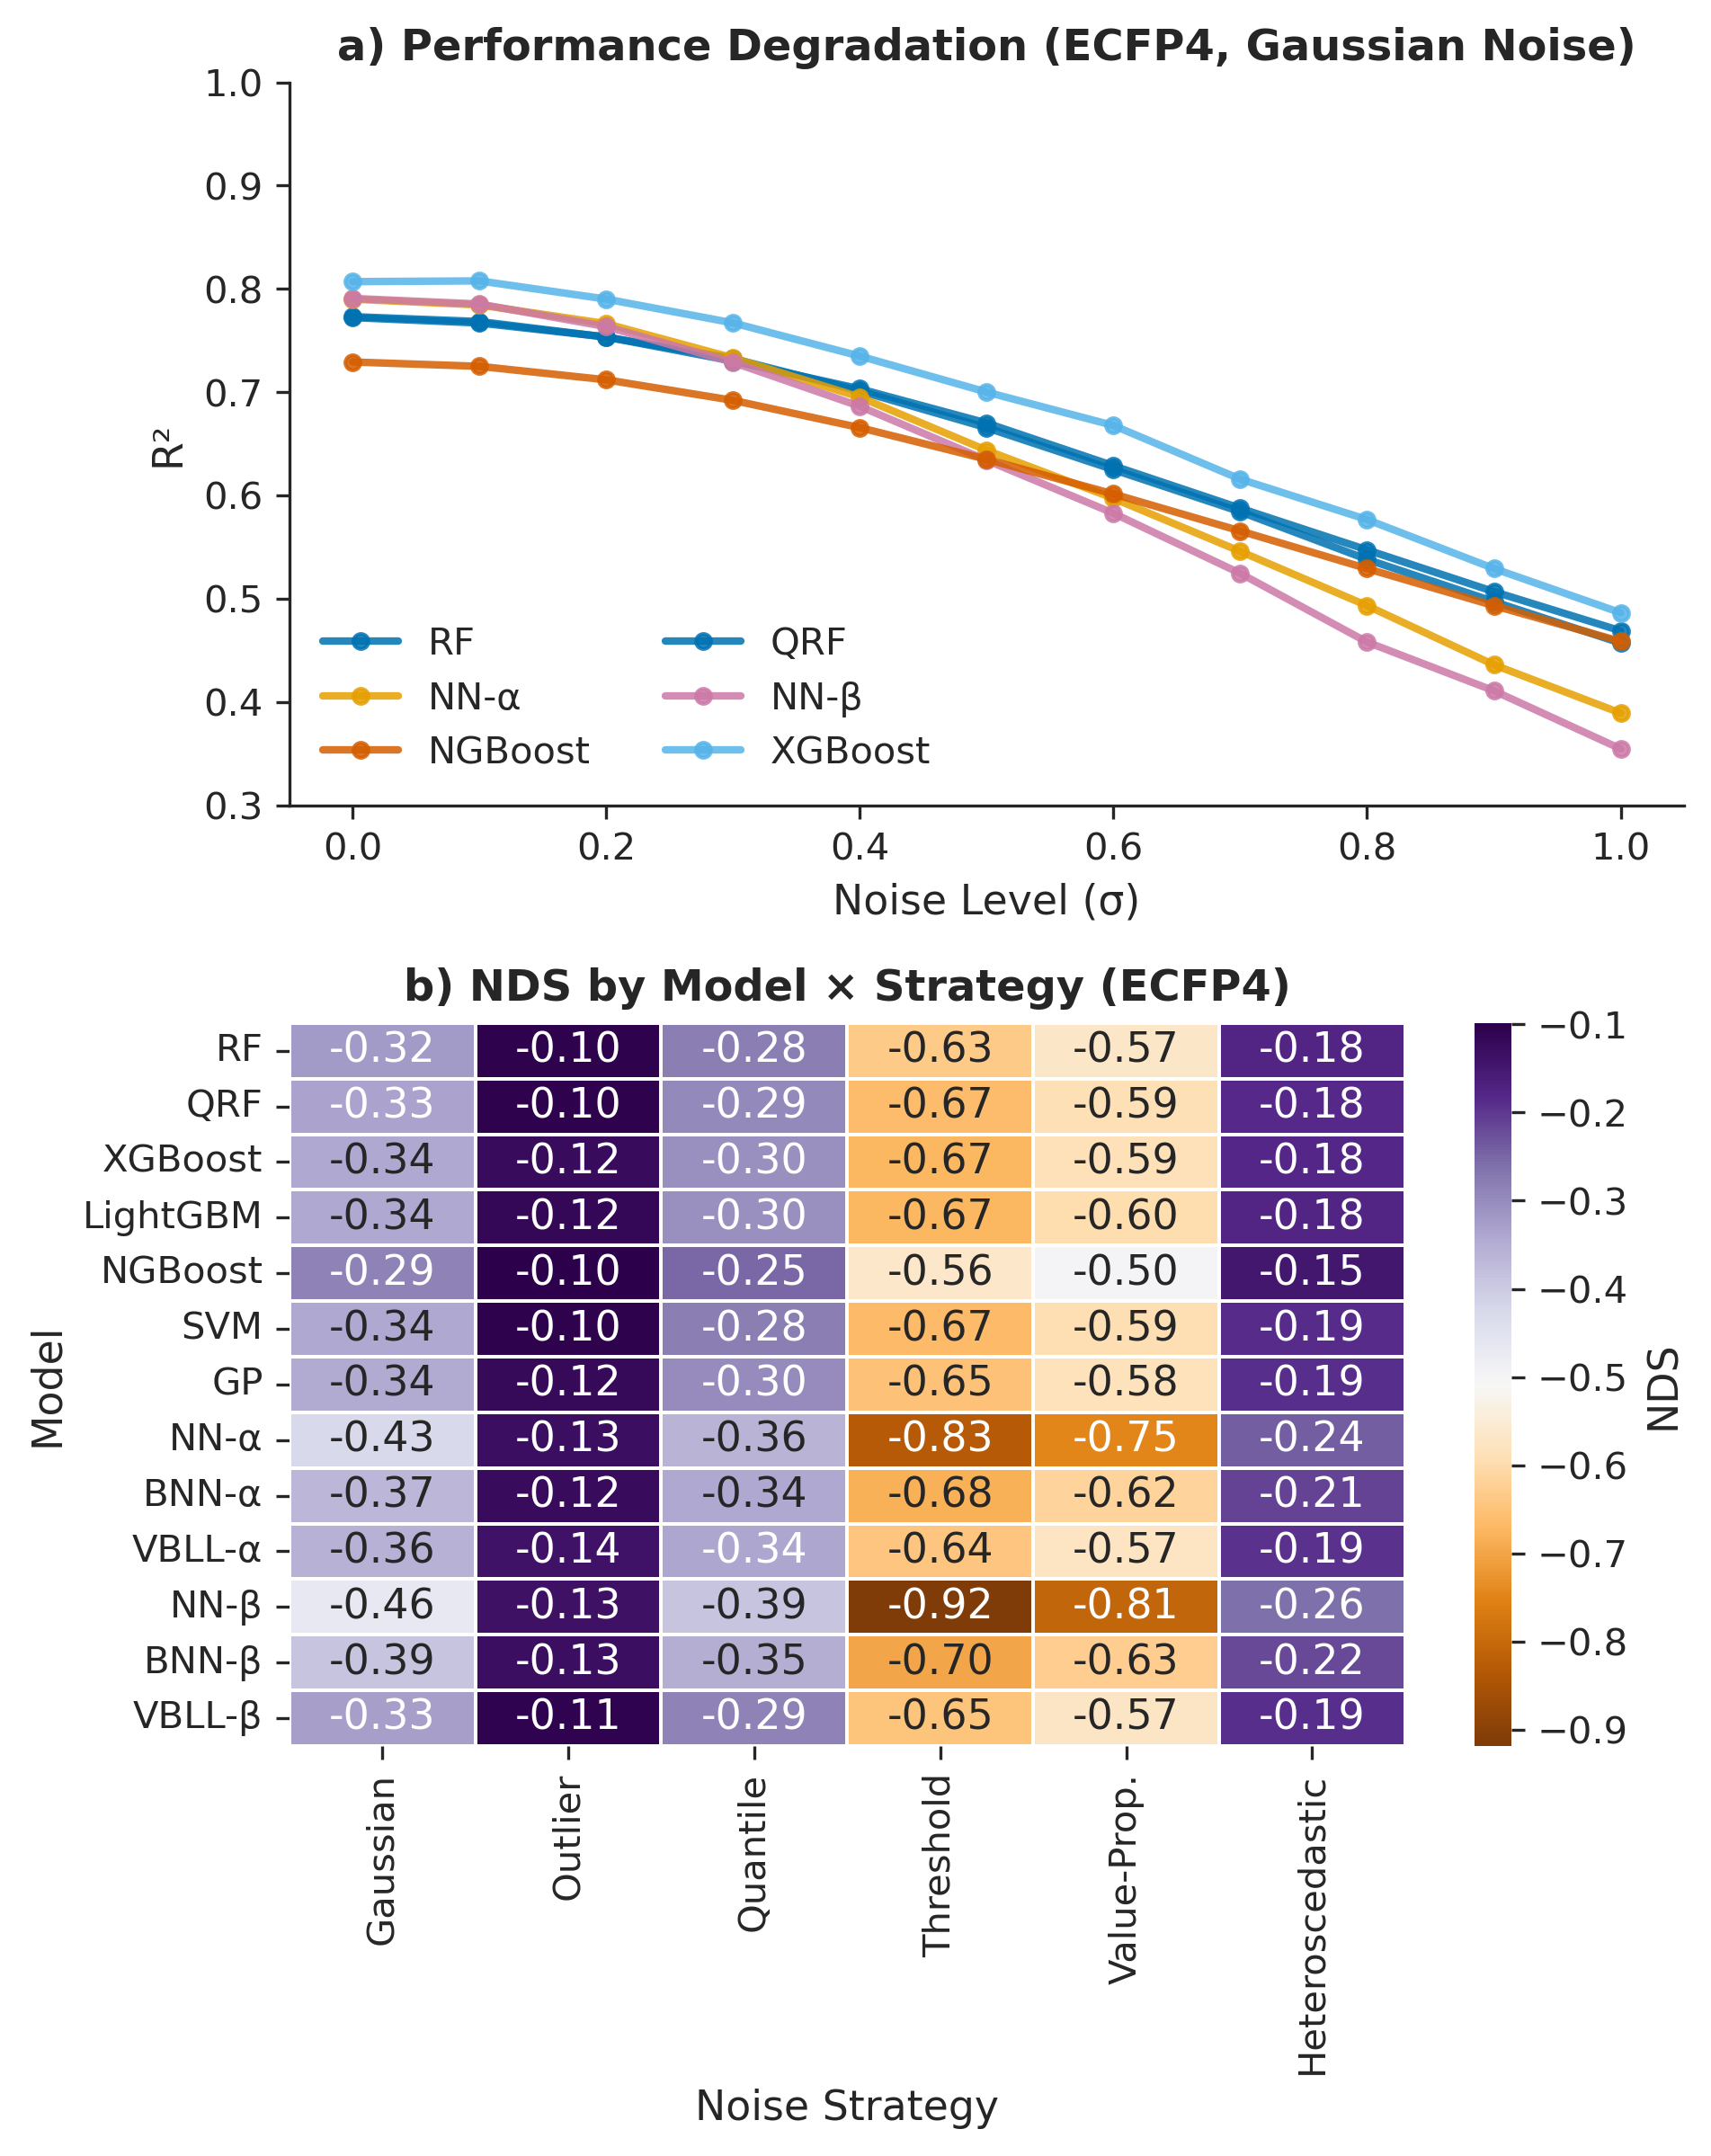
\includegraphics[width=\textwidth,height=0.78\textheight,keepaspectratio]{fig1_supp_ecfp4_overview.png}
\caption{\textbf{Figure S1: Global overview of noise robustness on the ECFP4 representation, evaluated on QM9 HOMO--LUMO gap.}
a) Performance degradation curves (R$^2$ versus noise level $\sigma$) under Gaussian noise. b) Noise degradation slope (NDS) heatmap across model architectures and noise strategies; lower (more negative) NDS indicates faster degradation under noise.}
\label{af6:ecfp4_overview}
\end{figure}

\newpage

%==============================================================================
% Additional file 7 — Baseline R^2 vs NDS scatter (was Supp Figure S2)
%==============================================================================

\begin{center}\Large\textbf{Additional file 7}\end{center}

\begin{figure}[H]
\centering
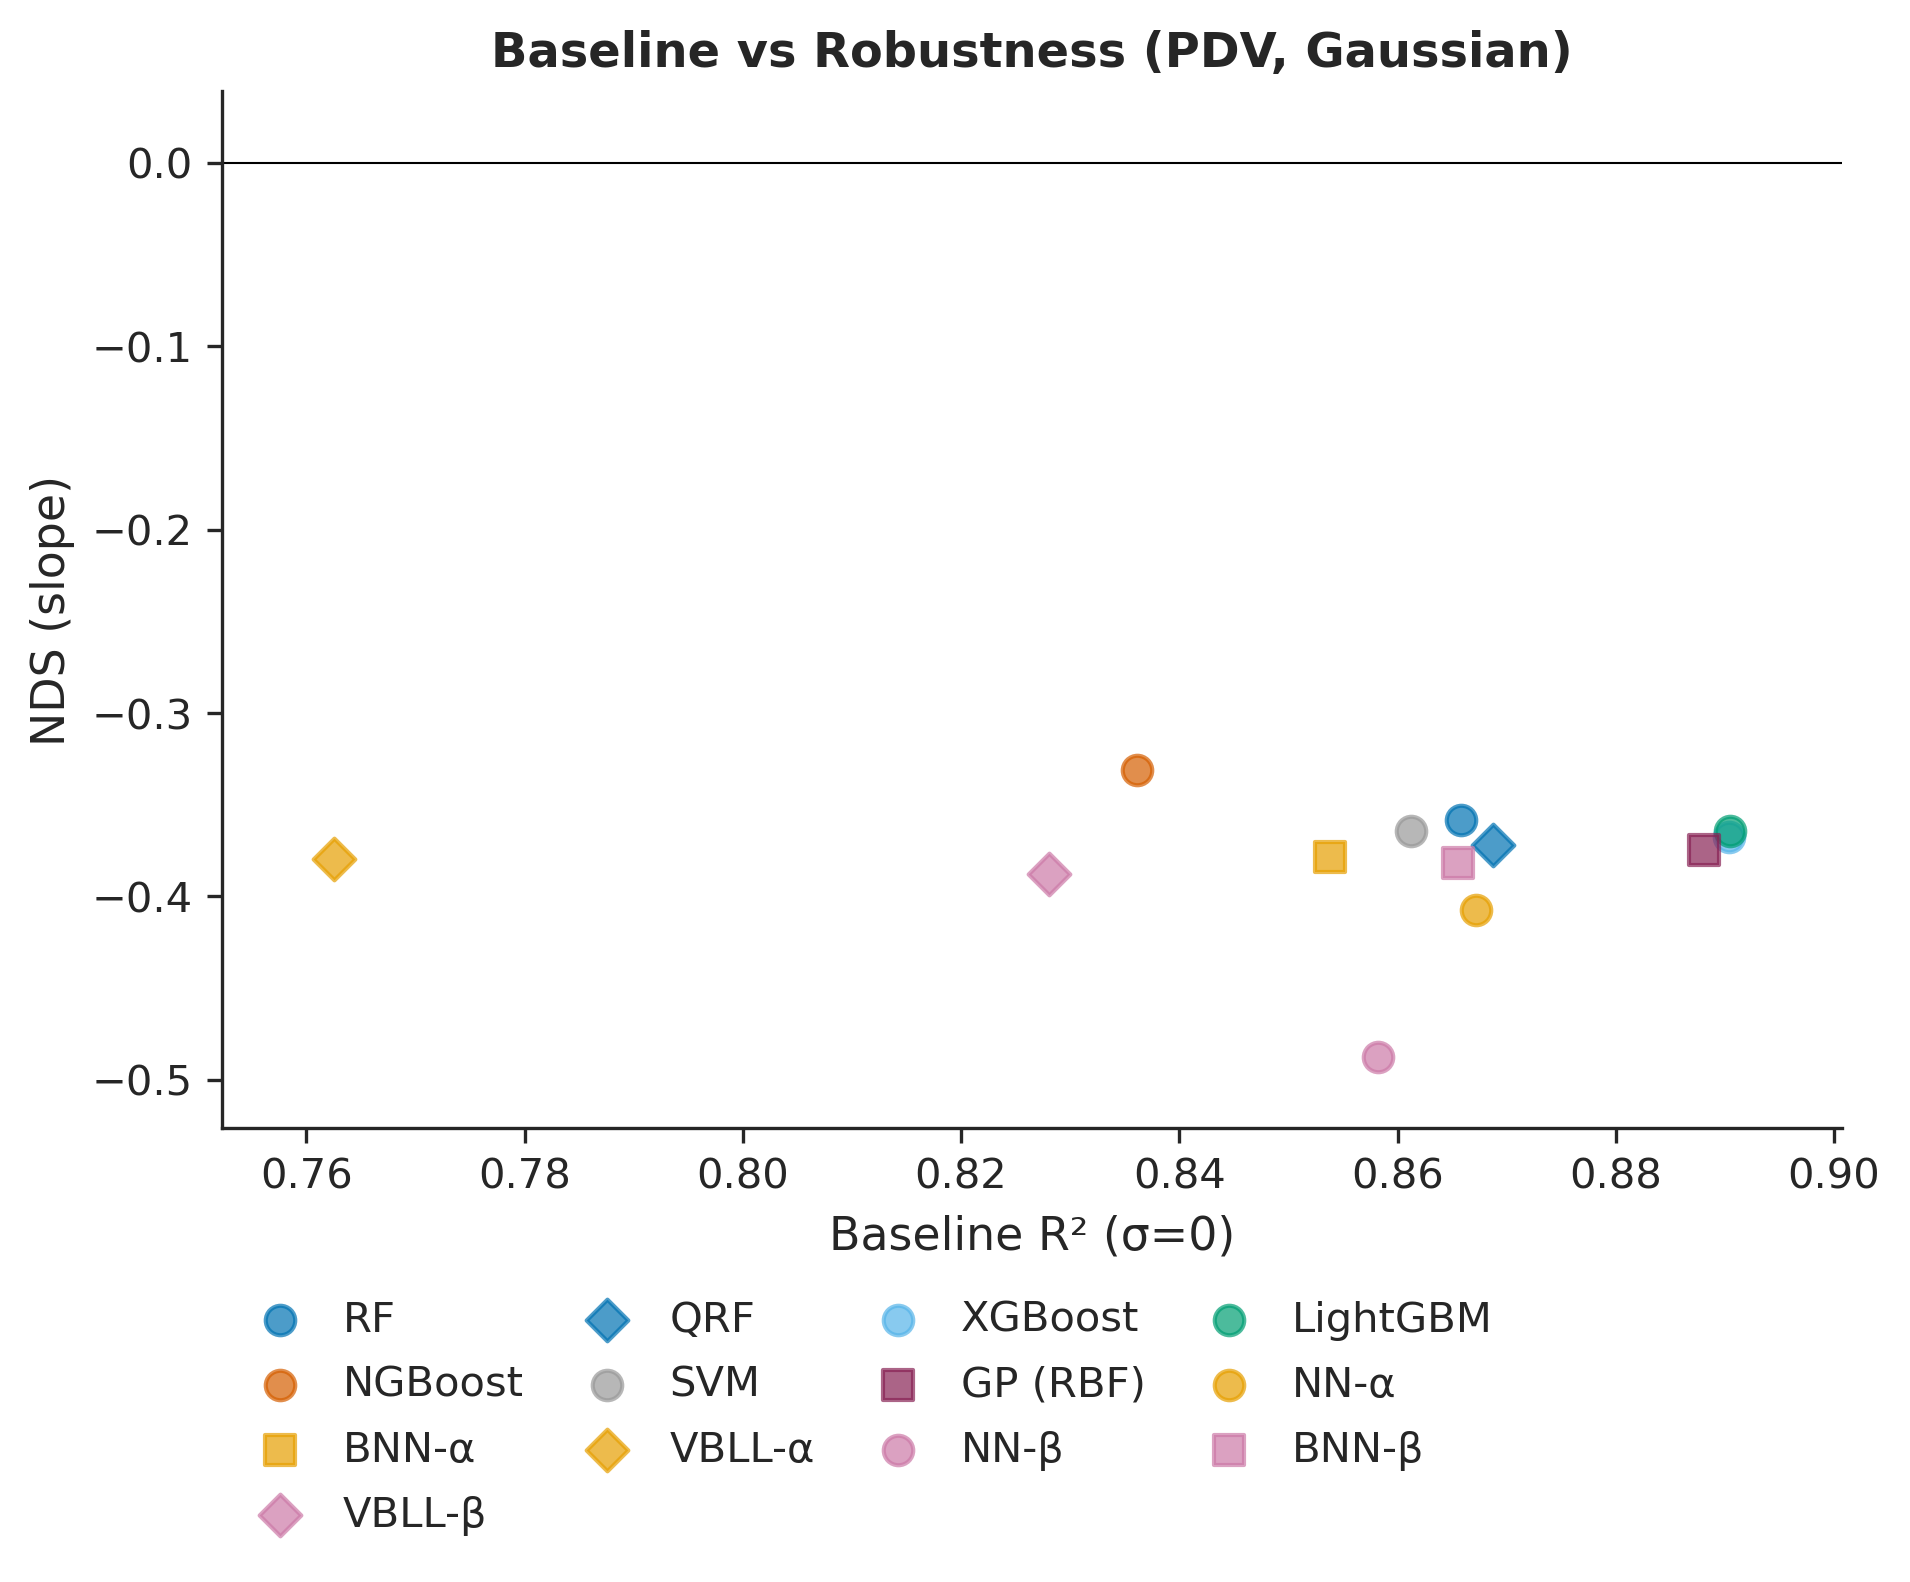
\includegraphics[width=\textwidth]{fig3_ranking_consistency.png}
\caption{\textbf{Figure S2: Baseline R$^2$ versus noise degradation slope (NDS) scatter for all models on the physicochemical descriptor vector (PDV) representation under Gaussian noise, on the QM9 HOMO--LUMO gap.}
Lower (more negative) NDS indicates faster performance loss under noise.}
\label{af7:ranking_consistency}
\end{figure}

\newpage

%==============================================================================
% Additional file 8 — NN Bayesian transformation effects (was Supp Table S6)
%==============================================================================

\begin{center}\Large\textbf{Additional file 8}\end{center}

\begin{table}[H]
\centering
\caption{\textbf{Table S6: Neural network Bayesian transformation effects on noise degradation slope (NDS) by representation, on the QM9 HOMO--LUMO gap.}
Positive $\Delta$ NDS indicates the Bayesian variant is more robust (less negative slope) than its deterministic counterpart.}
\label{af8:nn_transforms}
\small
\begin{tabular}{llrrrr}
\toprule
\textbf{Model} & \textbf{Representation} & \textbf{Baseline R$^2$} & \textbf{NN-$\beta$ NDS} & \textbf{BNN-$\beta$ NDS} & \textbf{$\Delta$ NDS} \\
\midrule
NN-$\beta$ & ECFP4 & 0.791 & $-0.464$ & $-0.388$ & $+0.076$ \\
NN-$\beta$ & PDV & 0.858 & $-0.487$ & $-0.382$ & $+0.106$ \\
NN-$\beta$ & SMILES & 0.721 & $-0.558$ & $-0.365$ & $+0.193$ \\
\bottomrule
\end{tabular}
\end{table}

\newpage

%==============================================================================
% Additional file 9 — Uncertainty metrics ECFP4 (was Supp Table S8)
%==============================================================================

\begin{center}\Large\textbf{Additional file 9}\end{center}

\begin{table}[H]
\centering
\caption{\textbf{Table S7: Uncertainty quantification metrics for probabilistic models on the ECFP4 representation (Gaussian noise strategy) on the QM9 HOMO--LUMO gap.}
Unc-Error $\rho$: Spearman correlation between predicted uncertainty and absolute prediction error. Unc-Noise $\rho$: Spearman correlation between predicted uncertainty and injected noise level $\sigma$. ECE: expected calibration error (lower = better-calibrated). Coverage targets: 68\% ($1\sigma$), 95\% ($2\sigma$).}
\label{af9:uncertainty_metrics}
\small
\begin{tabular}{lrrrrr}
\toprule
\textbf{Model} & \textbf{Unc-Error $\rho$} & \textbf{Unc-Noise $\rho$} & \textbf{ECE} & \textbf{Cov.\ $1\sigma$} & \textbf{Cov.\ $2\sigma$} \\
\midrule
\textbf{QRF}     & \textbf{0.25} & 0.27 & 0.19 & 74.7\% & 94.6\% \\
\textbf{NGBoost} & 0.22 & \textbf{0.37} & \textbf{0.11} & 69.2\% & 94.2\% \\
GP               & 0.18 & 0.34 & 0.23 & 78.6\% & 96.0\% \\
BNN-$\beta$      & 0.20 & 0.37 & 0.29 & 78.6\% & 95.2\% \\
BNN-$\alpha$     & 0.15 & 0.32 & 0.24 & 76.6\% & 95.1\% \\
VBLL-$\beta$     & 0.19 & 0.34 & 0.19 & 73.9\% & 95.5\% \\
VBLL-$\alpha$    & 0.11 & 0.31 & 0.22 & 74.5\% & 95.1\% \\
\bottomrule
\end{tabular}
\end{table}

\newpage

%==============================================================================
% Additional file 10 — Validation ANOVA (was Supp Figure S3)
%==============================================================================

\begin{center}\Large\textbf{Additional file 10}\end{center}

\begin{figure}[H]
\centering
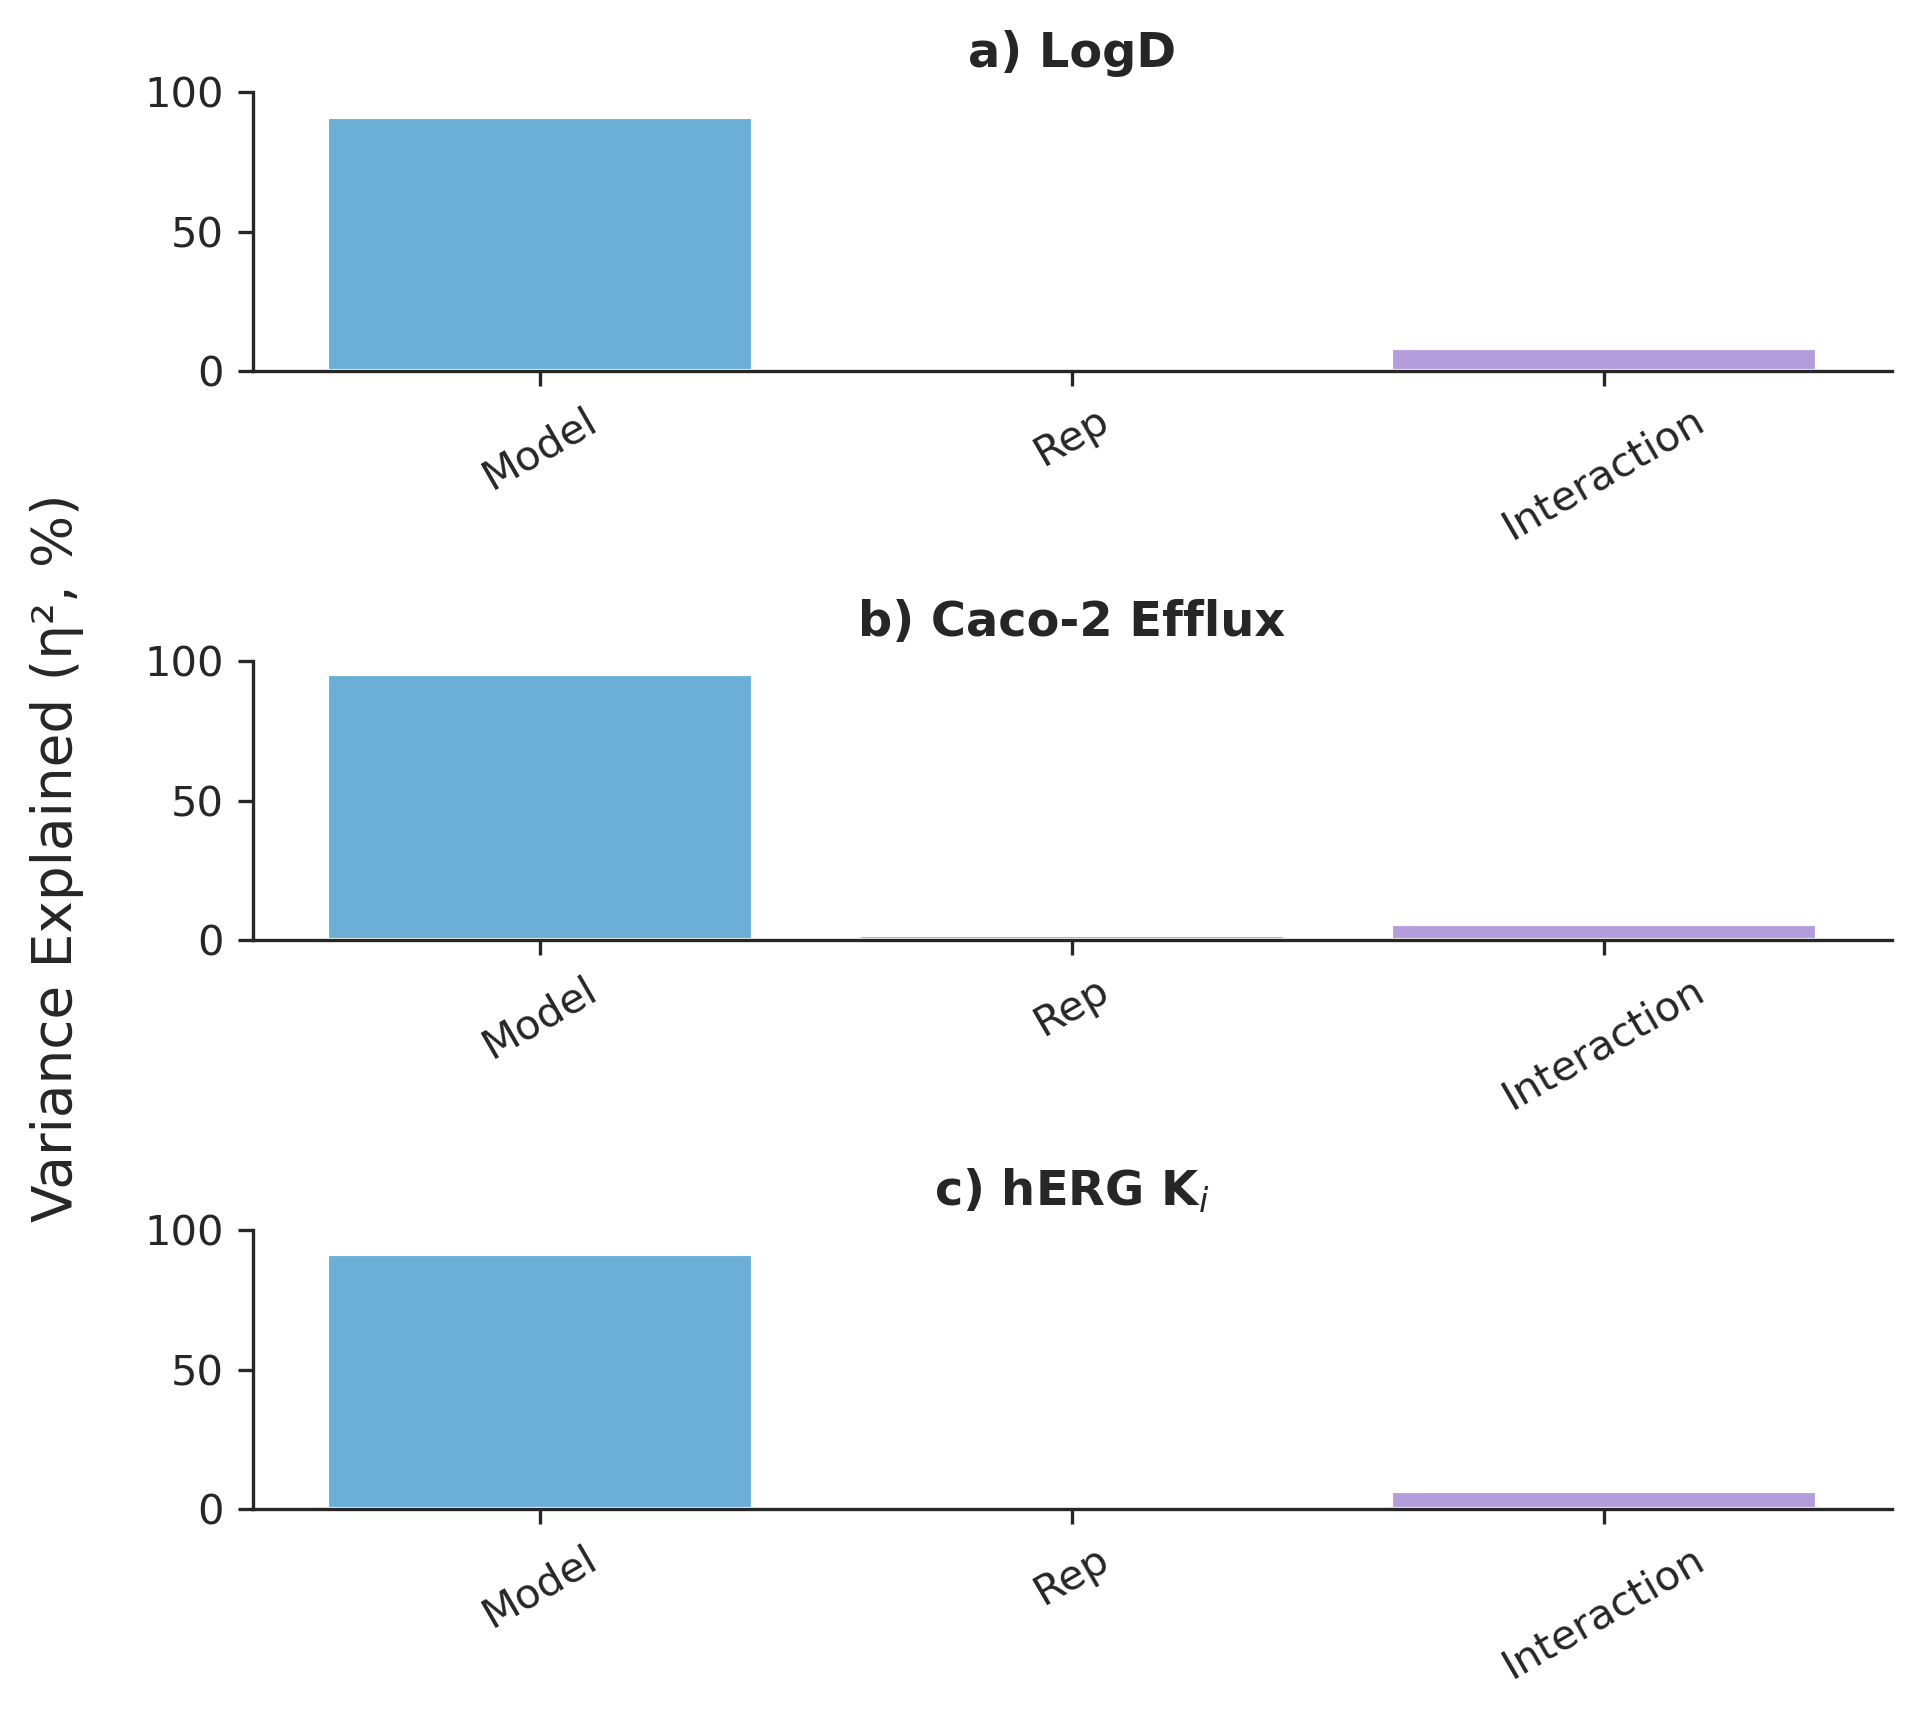
\includegraphics[width=\textwidth]{fig_validation_anova.png}
\caption{\textbf{Figure S3: ANOVA variance decomposition ($\eta^2$, \%) on external validation datasets: a) LogD, b) Caco-2 Efflux, and c) hERG K$_i$.}
Model, representation, and interaction contributions to noise degradation slope (NDS) variance for each dataset; lower (more negative) NDS indicates faster performance loss under noise.}
\label{af10:validation_anova}
\end{figure}

\newpage

%==============================================================================
% Additional file 11 — RF vs QRF on validation datasets (was Supp Table S7)
%==============================================================================

\begin{center}\Large\textbf{Additional file 11}\end{center}

\begin{table}[H]
\centering
\caption{\textbf{Table S8: Random forest (RF) vs quantile regression forest (QRF) noise degradation slope (NDS) on the three external validation datasets (LogD, Caco-2 Efflux, hERG K$_i$).}
Lower (more negative) NDS indicates faster degradation under noise.}
\label{af11:validation_rf_qrf}
\small
\begin{tabular}{lrrr}
\toprule
\textbf{Dataset} & \textbf{RF NDS} & \textbf{QRF NDS} & \textbf{$\Delta$ NDS} \\
\midrule
ChEMBL-hERG-Ki     & $-0.231$ & $-0.359$ & $-0.128$ \\
OpenADMET-Caco2    & $-0.534$ & $-0.627$ & $-0.094$ \\
OpenADMET-LogD     & $-0.101$ & $-0.185$ & $-0.083$ \\
\bottomrule
\end{tabular}
\end{table}


\end{document}
